%!TEX TS-program = XeLaTeX

%!TEX TS-program = XeLaTeX
\documentclass[11pt]{article}

\usepackage{amssymb}
\usepackage{amsthm}
\usepackage{amsmath}
\usepackage{mathtools}

\usepackage{fancyhdr}
\usepackage{graphicx}
\usepackage[top=3cm, left=2cm, right=2cm, headheight = 90pt]{geometry}
\usepackage{xltxtra}
\usepackage[font=small,labelfont=bf]{caption}

\usepackage{multicol}

\renewcommand{\theenumi}{\alph{enumi}}


\def\leq{\leqslant}
\def\geq{\geqslant}
\def\N{\mathbb N}
\def\R{\mathbb R}
\def\Z{\mathbb Z}
\DeclarePairedDelimiter\set\{\}

\def\prob{}

\theoremstyle{definition}
\newtheorem{problem}{\prob}


\pagestyle{fancy}

%!TEX TS-program = XeLaTeX
\renewcommand{\figurename}{Attēls}


\fancyhead[C]{{\Large\bf Strategies and tactics - Problems}\\ \date}

\begin{document}
%\thispagestyle{fancy}
\noindent 
%\emph{\notes}

%1
\begin{problem}
\textit{[Tilta problēma - "neiespējamības barjera, paplašināšanas metode"]}
Četri cilvēki tumšā naktī bēg no briesmīgām šausmām un nonāk pie aizas, kurai vienīgais ceļš pāri ir šaurs virvju tilts. Uz tilta vinlaicīgi var atrasties ne vairāk kā divi cilvēki. Tā kā ir tumšs, tad uz tilta nevar atrasties cilvēks bez lukturīša tiešā tuvumā, un lukturītis uz visiem ir viens (bet divi cilvēki var pāriet pāri tiltam ar vienu lukturīti).  
Šiem cilvēkiem ir dažāds līmenis bailēm no tumsas un augstuma, līdz ar to viņu pārvietošanās ātrums pa tiltu ir dažāds - $1$, $2$, $5$ un $10$ minūtes, lai pārietu tiltam vienā virzienā. Ja divi cilvēki iet pāri tiltam kopā, viņi kustās lēnākā cilvēka ātrumā.
Papildus tam visam tilts ir mīnēts un sabruks pēc precīzi $18$ minūtēm,

Vai visi četri cilvēki var veiksmīgi nonākt otrā pusē?
\begin{center}
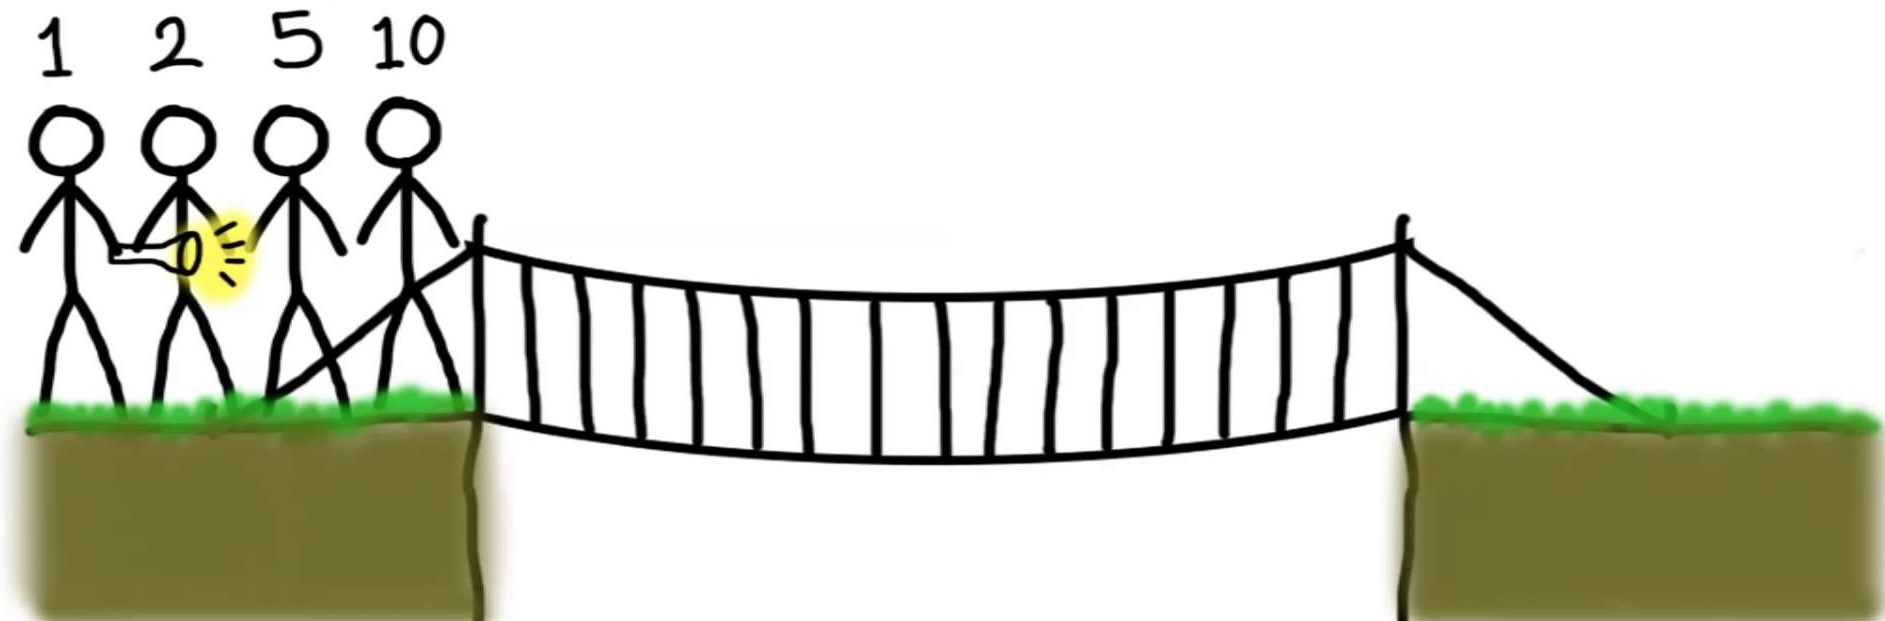
\includegraphics[width=5cm]{bridge.jpg}
\captionof{figure}{Tilts pāri aizai}
\label{fig:bridge}
\end{center}
\end{problem}
%

%2
\begin{problem}
\textit{[9 dots - "thinking outside the box"]}
$9$ dots are drawn in a $3 \times 3$ grid on a piece of paper. Can you draw $4$ straight, continuous lines that connect all the dots, without lifting the pencil from the paper?
\begin{center}

\includegraphics[width=2cm]{3by3.jpg}
\captionof{figure}{9 dots}
\label{fig:bridge}
\end{center}
\end{problem}
%

%3
\begin{problem}
\textit{[More dots - "reduction","thinking outside the box"]}
Same as previous problem, but with:
\begin{enumerate}
\item $5 \times 5$ with $8$ lines 
\item $4 \times 4$ with $6$ lines
\item $3 \times 4$ with $5$ lines
\item $4 \times 5$ with $7$ lines
\end{enumerate}
\end{problem}
%

%4
\begin{problem}
\textit{[Sultan's law - "symmetry"]}
There is equal amount of men and women in Arabia, but, for religious reasons, Sultan would wish it that there would be more women than men. 

He decides on the following law: each couple has to keep having children until a first son is born and then stop having children. How well would this law work? What would be the average size of family with this law?
\end{problem}
%


%5
\begin{problem}
\textit{[Gambling problem - "symmetry"]}
Elize and Rudolf were bored during a class and decided to play a gambling game. They have a fair coin, but instead of keeping it simple they decided on a following game: first each of them chose a $3$ event string (for example "heads-heads-tails"). Then they start tossing a coin and write down results until they encounter one of the chosen substrings, which then is the winner. Decide if the game is fair for the following:
\begin{enumerate}
\item "heads-heads-heads" vs "tails-tails-tails"
\item "heads-heads-heads" vs "heads-heads-tails"
\item "tails-tails-heads" vs "heads-heads-tails"
\item "tails-tails-heads" vs "heads-heads-heads"
\end{enumerate}

\end{problem}
%
\end{document}
